%
%
\documentclass[11pt,french,english]{article}
\usepackage[T1]{fontenc}
\usepackage[utf8]{inputenc}
\usepackage{amssymb}
\usepackage{amsmath}
\usepackage{ulem}
\usepackage{url}
\usepackage{graphicx}
\usepackage{enumitem}
\usepackage{bm}


\makeatletter

%
\providecommand{\LyX}{L\kern-.1667em\lower.25em\hbox{Y}\kern-.125emX\@}

\makeatother

\usepackage{lmodern}
\usepackage[english]{babel}
\makeatletter
\addto\extrasfrench{%
   \providecommand{\og}{\leavevmode\flqq~}%
   \providecommand{\fg}{\ifdim\lastskip>\z@\unskip\fi~\frqq}%
}

\makeatother



\usepackage[colorinlistoftodos]{todonotes}

\usepackage{todonotes}
\newcommand{\ioannis}[1]{\todo[inline,color=green!40,caption={}]{{\it Ioannis:~}#1}}
\newcommand{\guillaume}[1]{\todo[inline,color=blue!40,caption={}]{{\it Guillaume:~}#1}}

\newcommand{\gradpoints}[1]{\textcolor{red}{Graduates #1 pts}}
\newcommand{\undergradpoints}[1]{\textcolor{orange}{Undergraduates #1 pts}}


\newcommand{\french}[1]{ {\color{blue} #1} }


%
\usepackage{etoolbox}
\providetoggle{undergrad}
\settoggle{undergrad}{true}
\providetoggle{grad}
\settoggle{grad}{false}
%
%
%

%
\newcommand{\points}[2]{\iftoggle{undergrad}{{\color{red}[#1 points]}}{\color{red}[#1 points]}}
%
%

\usepackage[colorlinks=true]{hyperref}

\newcommand{\blue}[1]{{\color{blue}#1}}
\newcommand{\ith}[1]{^{(#1)}}

%



\renewcommand{\vec}[1]{{\bf #1}}
\newcommand{\mat}[1]{{\bf #1}}
\newcommand{\ten}[1]{\mat{\ensuremath{\boldsymbol{\mathcal{#1}}}}}
\newcommand{\mats}[1]{\ensuremath{\mathbf{\boldsymbol{#1}}}}
\newcommand{\vecs}[1]{\ensuremath{\mathbf{\boldsymbol{#1}}}}


\newcommand{\loss}{\ell}

\newcommand{\sigmoid}{\sigma}
\providecommand{\alert}[1]{{\color{MyRed}#1}}


\newcommand{\x}{\vec{x}}
\newcommand{\y}{\vec{y}}
\newcommand{\z}{\vec{z}}
\renewcommand{\u}{\vec{u}}
\renewcommand{\v}{\vec{v}}
\newcommand{\vmu}{\vecs{\mu}}
\newcommand{\w}{\vec{w}}
\newcommand{\X}{\mat{X}}
\newcommand{\Y}{\mat{Y}}
\newcommand{\W}{\mat{W}}
\newcommand{\K}{\mat{K}}
\newcommand{\I}{\mat{I}}
\newcommand{\M}{\mat{M}}
\newcommand{\U}{\mat{U}}
\newcommand{\D}{\mat{D}}
\newcommand{\A}{\mat{A}}
\newcommand{\B}{\mat{B}}
\renewcommand{\H}{\mat{H}}
\renewcommand{\S}{\mat{S}}
\renewcommand{\b}{\vec{b}}
\renewcommand{\a}{\vec{a}}
\newcommand{\MPhi}{\mats{\Phi}}
\newcommand{\Mphi}{\mats{\Phi}}

\DeclareMathOperator*{\Prob}{\mathbb{P}}
\DeclareMathOperator*{\Esp}{\mathbb{E}}
\newcommand{\ind}{\mathrm{I}}

%
\newcommand{\T}{\ten{T}}
\newcommand{\ttm}[1]{\times_{#1}}
%
\newcommand{\ttv}[1]{\bullet_{#1}}
%
\newcommand{\tenmat}[2]{\mat{#1}_{(#2)}}
\newcommand{\tenmatpar}[2]{(#1)_{(#2)}}

%
\newcommand{\kron}{\otimes}
\newcommand{\krao}{\odot}
\newcommand{\hadam}{*}
\newcommand{\outprod}{\otimes}
\newcommand{\dirsum}{\oplus}

%
\newcommand{\Xcal}{\mathcal{X}}
\newcommand{\Dcal}{\mathcal{D}}
\newcommand{\Lcal}{\mathcal{L}}
\newcommand{\Hcal}{\mathcal{H}}
\newcommand{\Scal}{\mathcal{S}}
\newcommand{\Rcal}{\mathcal{R}}
\newcommand{\Fcal}{\mathcal{F}}
\newcommand{\Ncal}{\mathcal{N}}
\newcommand{\Ycal}{\mathcal{Y}}
\newcommand{\R}{\mathbb{R}}

\newcommand{\Rbb}{\mathbb{R}}

%


\newcommand{\bmat}[1]{\left[\begin{matrix}
#1
\end{matrix}\right]}


\newcommand{\sign}{\mathrm{sign}}
\newcommand{\inv}{^{-1}}
\DeclareMathOperator*{\Tr}{Tr} %
\DeclareMathOperator*{\argmax}{arg\,max}
\DeclareMathOperator*{\argmin}{arg\,min}
\newcommand{\vectorize}[1]{\mathrm{vec}(#1)}
\DeclareMathOperator*{\reshape}{reshape}
\newcommand{\eqdef}{\triangleq}
\newcommand{\vtimes}[1]{\ \overline{\times}_{#1}\ }
\DeclareMathOperator*{\rank}{rank}
\newcommand{\norm}[1]{\|#1\|}
\newcommand{\Ker}{\mathrm{Ker}}
\renewcommand{\Im}{\mathrm{Im}}
\newcommand{\bigo}[1]{\mathcal{O}\left(#1\right)}
\newcommand{\singv}{\mathfrak{s}}
\newcommand{\vspan}[1]{span(#1)}
\newcommand{\dotprod}[2]{\langle #1, #2\rangle} 
\begin{document}

\setlength{\parskip}{0.3cm} \setlength{\parindent}{0cm}

\begin{center}
\textbf{IFT-3395 Fundamentals of Machine Learning} \\
\textbf{Professor: Guillaume Rabusseau }
\par\end{center}{\large \par}

\begin{center}
\textbf{\LARGE{Homework 2 - Theoretical part}} \\
\textbf{\textcolor{blue}{Devoir 2 - Partie Th\'eorique}}
\par\end{center}{\LARGE \par}


%


%


%
\paragraph{}
\begin{itemize}
\item This homework must be done and submitted to Gradescope and can be done in groups of at most \iftoggle{undergrad}{2}{2} students.
You are welcome to discuss with students outside of your group  \emph{but the solution submitted by a group must be its own}.
Note that we will use Gradescope's plagiarism detection feature.
All suspected cases of plagiarism will be recorded and shared with university officials for further handling.\\
\french{Ce devoir doit être déposé sur Gradescope  et peut être fait en équipes de \iftoggle{undergrad}{2}{2} étudiants maximum. Vous pouvez discuter avec des étudiants d'autres groupes  \emph{mais les réponses soumises par le groupe doivent être originales}. A noter que nous utiliserons l'outil de détection de plagiat de Gradescope. Tous les cas suspectés de plagiat seront enregistrés et transmis à l'Université pour vérification.}

\item You need to submit your solution as a pdf file on Gradescope using the homework titled 
\iftoggle{undergrad}{\texttt{(3395: UNDERGRAD) Theoretical Homework 2}}{\texttt{(6390: GRAD) Theoretical Homework 2}}.
\\
\french{Vous devez soumettre vos solutions au format pdf sur Gradescope en utilisant le devoir intitulé \iftoggle{undergrad}{\texttt{(3395: UNDERGRAD) Theoretical Homework 2}}{\texttt{(6390: GRAD) Theoretical Homework 2}}.}
\end{itemize} 
\begin{enumerate}
%
\item{  \textbf{Bias-Variance decomposition}
\french{Décomposition biais/variance}
\points{5}{2}



Consider the following data generation process: an input point $x$ is drawn from an unknown distribution and the output $y$ is generated using the formula 
$$
y = f(x) + \epsilon,
$$
where $f$ is an unknown deterministic function and $\epsilon \sim \mathcal{N}(\mu,\,\sigma^{2})$. This  process implicitly defines a distribution over inputs and outputs; we denote this distribution by $p$.

Given an i.i.d. training dataset $D=\{({x}_1, y_1),\dots,({x}_n, y_n)\}$ drawn from $p$, we can fit the hypothesis $h_D$ that minimizes the empirical risk with the squared error loss function. More formally,
$$
h_D= \argmin_{h\in \mathcal H}  \sum_{i=1}^n (y_i - h({x}_i))^2
$$
where $\mathcal H$ is the set of hypotheses (or function class) in which we look for the best hypothesis/function.

The expected error\footnote{Here the expectation is over random draws of the training set $D$ of $n$ points from the unknown distribution $p$. For example (and more formally): $\Esp[(h_D({x'})] = \Esp_{(x_1,y_1)\sim p} \cdots \Esp_{(x_n,y_n)\sim p} \Esp[(h_{\{({x}_1, y_1),\dots,({x}_n, y_n)\}}({x'})]$.}  of $h_D$ on a fixed data point $(x',y')$ is given by $\Esp[(h_D({x'}) - y')^2]$. We will show that this error can be decomposed as a function of two meaningful terms:
\begin{itemize}
    \item The \emph{bias}, which is the difference between the expected value of hypotheses at ${ x}'$ and the true value  $f({x'})$. Formally,
$$
\textit{bias}= \Esp[h_D({x'})]-f({x'})
$$
\item The \emph{variance}, which is how far hypotheses learned on different datasets are spread out from their mean $\Esp[h_D({x'})]$. Formally,
$$
\textit{variance}= \Esp[(h_D({x'}) - \Esp[h_D({x'})])^2]
$$
\end{itemize}


Show that the expected prediction error on $({x'},y')$ can be decomposed into a sum of 3 terms: $(\textit{bias})^2$, $\textit{variance}$, and a $\textit{noise}$ term involving $\epsilon$. You need to justify all the steps in your derivation.

\french{

Considérons les données générées de la manière suivante: une donnée $x$ est échantillonnée à partir d'une distribution inconnue, et nous observons la mesure correspondante $y$ générée d'après la formule
$$
y = f(x) + \epsilon,
$$
où $f$ est une fonction déterministe inconnue et  $\epsilon \sim \mathcal{N}(\mu,\,\sigma^{2})$. Ceci définit une distribution sur les données $x$ et mesures $y$, nous notons cette distribution $p$.

Étant donné un ensemble d'entraînement $D=\{({x}_1, y_1),\dots,({x}_n, y_n)\}$ échantillonné i.i.d. à partir de $p$, on définit l'hypothèse $h_D$ qui minimise le risque empirique donné par la fonction de coût erreur quadratique. Plus précisément,
$$
h_D= \argmin_{h\in \mathcal H}  \sum_{i=1}^n (y_i - h({x}_i))^2
$$
où $\mathcal H$ est l'ensemble d'hypothèses (ou classe de fonction) dans lequel nous cherchons la meilleure fonction/hypothèse.

L'erreur espérée\footnote{\french{Ici l'espérance porte sur le choix aléatoire d'un ensemble d'entraînement $D$ de $n$ points tirés à partir de la distribution inconnue $p$. Par exemple (et plus formellement) : $\Esp[(h_D({x'})] = \Esp_{(x_1,y_1)\sim p} \cdots \Esp_{(x_n,y_n)\sim p} \Esp[(h_{\{({x}_1, y_1),\dots,({x}_n, y_n)\}}({x'})]$.}  } de $h_D$ sur un point donné $(x',y')$ est notée $\Esp[(h_D({x'}) - y')^2]$. Nous allons montrer que cette erreur peut être décomposée en deux termes importants:
\begin{itemize}
    \item Le \emph{biais}, qui est la différence entre l'espérance de la valeur donnée par notre hypothèse en un point ${ x}'$ et la vraie valeur donnée par  $f({x'})$. Plus précisément,
$$
\textit{biais}= \Esp[h_D({x'})]-f({x'})
$$
\item La \emph{variance}, est une mesure de la dispersion des hypothèse apprises sur des ensemble de données différents, autour de la moyenne $\Esp[h_D({x'})]$. Plus précisément,
$$
\textit{variance}= \Esp[(h_D({x'}) - \Esp[h_D({x'})])^2]
$$
\end{itemize}

Montrez que l'erreur espérée pour un point donné $({x'},y')$ peut être décomposée en une somme de 3 termes: $(\textit{biais})^2$, $\textit{variance}$, et un terme de $\textit{bruit}$ qui implique $\epsilon$. Vous devez justifier toutes les étapes de dérivation.
}
}
 %

\item{ {\bf Feature Maps}
\french{Fonctions de transformation des données}
\points{8}{8}


In this exercise, you will design feature maps to transform an original dataset into a linearly separable set of points. For the following questions, if your answer is `\textit{yes}', write the expression for the proposed transformation; and if your answer is `\textit{no}', write a brief explanation. You are expected to provide explicit formulas for the feature maps, and these formulas should only use common mathematical operations.

\french{Dans cet exercice, vous allez concevoir des fonctions de transformation depuis l'espace de traits caractéristiques original vers un espace où les données sont linéairement séparables. Pour les questions suivantes, si vous répondez `\textit{oui}', écrivez l'expression de la transformation correspondante; et si votre réponse est `\textit{non}', ajoutez une courte justification de votre réponse. Vous devez donner les formules explicites des transformations, et ces formules doivent utiliser uniquement des opérations mathématiques simples.
}


\begin{enumerate}
    \item { [2 points] Consider the following 1-D dataset (Figure \ref{a}). Can you propose a 1-D transformation that will make the points linearly separable? \french{ Soit les données 1-D suivantes (Figure \ref{a}). Pouvez-vous proposer une transformation 1-D (i.e. vers un espace de dimension 1) qui rend les points linéairement séparables?}

    \begin{figure}[!h]
    \centering
    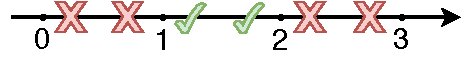
\includegraphics[width=0.55\textwidth]{homework2/img/feat_map.pdf}
    \caption{}
    \label{a}
    \end{figure}}
%

    \item { [2 points] Consider the following 2-D dataset (Figure \ref{b}). Can you propose a 1-D transformation that will make the data linearly separable? \french{Soit les données 2-D suivantes (Figure \ref{b}). Pouvez-vous proposer une transformation 1-D qui rend les points linéairement séparables?}
    \begin{figure}[h]
    \centerline{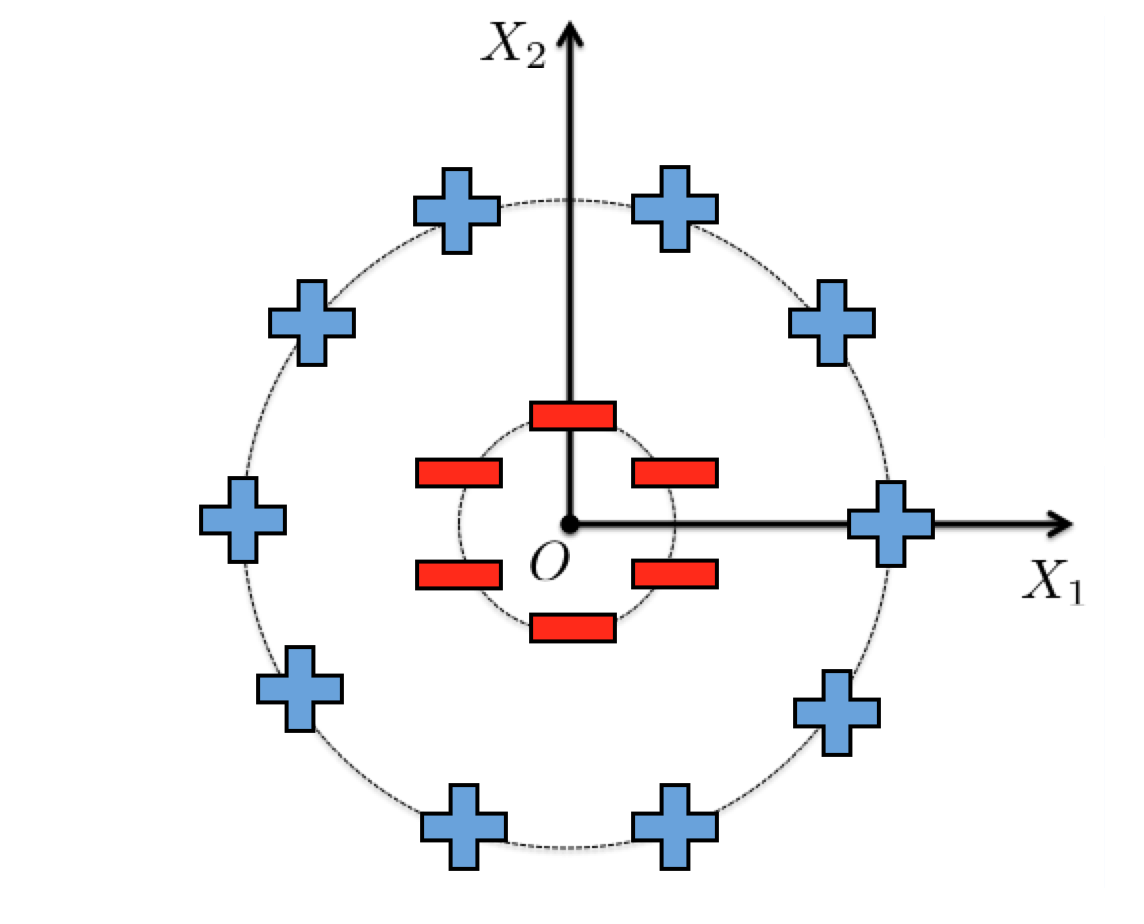
\includegraphics[scale=0.4]{homework2/img/D5.png}}
    \caption{}
    \label{b}
    \end{figure}}

    \item { [4 points] Using ideas from the above two datasets, can you suggest a 2-D transformation of the following dataset (as shown in Figure \ref{12}) that makes it linearly separable? If `\textit{yes}', also provide the kernel corresponding to the feature map you proposed. \french{En utilisant les idées que vous avez utilisées pour les deux questions précédentes, pouvez-vous proposer une transformation 2-D des données suivantes (Figure \ref{12}) qui les rendent linéairement séparables? Si votre réponse est `\textit{oui}', donnez l'expression du noyau qui correspond à la transformation proposée.}
    \begin{figure}[ht]
    \centering
    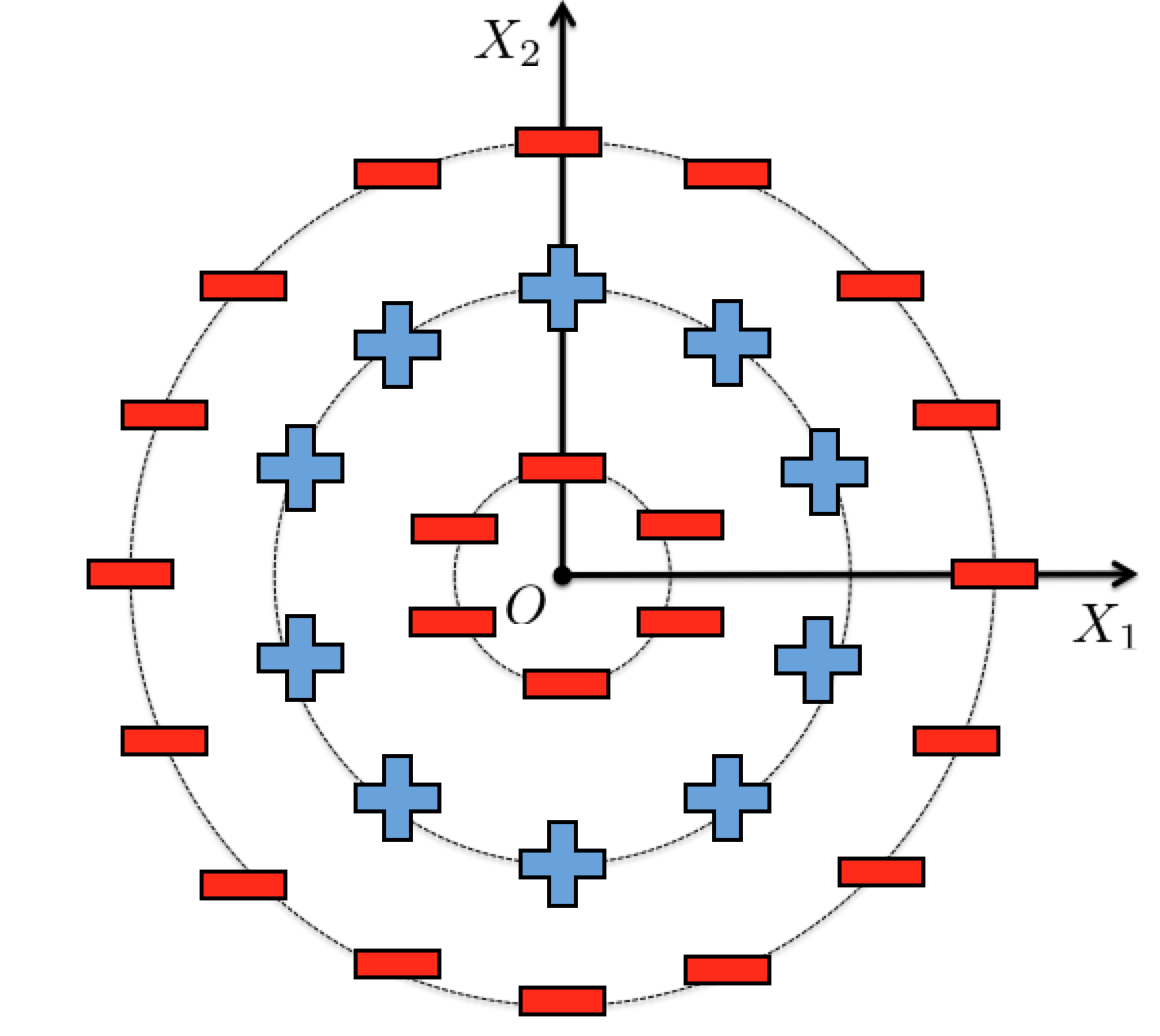
\includegraphics[scale=0.3]{homework2/img/D6.png}
    \caption{}
    \label{12}
    \end{figure}}
\end{enumerate} 
}
 %

\item \textbf{Optimization} \french{Optimisation}
\points{15}{10}

    Assume a quadratic objective function of the form: 
    $$
        f(x) = \frac{1}{2} x^T A x + x^T b + a,
    $$
    where $x \in \mathbb{R}^d$,
    $b \in \mathbb{R}^d$,
    $a \in \mathbb{R}$ and $A$ is a $d \times d$ symmetric, positive definite matrix.
    This means that the matrix $A$ admits the eigendecomposition $A=U \Lambda U^T$,
    where $U \in \mathbb{R}^{d \times d}$ is an orthonormal matrix and $\Lambda  \in \mathbb{R}^{d \times d}$ is a diagonal matrix.
    The $i$-th column vector of $U$, denoted by $u_i \in \mathbb{R}^d$, represents the $i$-th eigenvector of $A$.
    The $i$-th diagonal element of $\Lambda$, denoted by $\lambda_i \in \mathbb{R}$, represents the $i$-th eigenvalue of $A$.
    We will assume here that all eigenvalues are unique. 
    Furthermore, without loss of generality, the eigenvectors and eigenvalues in the decomposition can be ordered in such a way that
    $$
        \lambda_1 > \lambda_2 > \ldots
        > \lambda_d > 0.
    $$

\french{    Soit la fonction objectif suivante: 
    $$
        f(x) = \frac{1}{2} x^T A x + x^T b + a,
    $$
    où $x \in \mathbb{R}^d$,
    $b \in \mathbb{R}^d$,
    $a \in \mathbb{R}$ et $A$ est une matrice $d \times d$ symétrique, positive définie.
    Ceci implique que la matrice $A$ admet la décomposition en valeur propres $A=U \Lambda U^T$,
    où $U \in \mathbb{R}^{d \times d}$ est une matrice orthogonale et $\Lambda  \in \mathbb{R}^{d \times d}$ est une matrice diagonale.
    La $i$-ème colonne de $U$, noté $u_i \in \mathbb{R}^d$, représente le $i$-ème vecteur propre de $A$.
    Le $i$-ème élément diagonal de $\Lambda$, noté $\lambda_i \in \mathbb{R}$, représente la $i$-ème valeur propre de $A$. Nous supposons que toutes les valeurs propres sont uniques. De plus, sans perte de généralité, les vecteurs propres et valeurs propres peuvent être ordonnés de manière à avoir
    $$
        \lambda_1 > \lambda_2 > \ldots
        > \lambda_d > 0.
    $$
}
    
\begin{enumerate}
    \item Find all of the stationary points of $f(x)$ analytically, i.e. through a closed-form expression (Justify). \french{Donnez une expression analytique pour tous les points stationnaires de $f(x)$, en justifiant votre réponse.}
    \item Which of those stationary points are minima, maxima and saddle-points?
    Give a mathematically rigorous explanation why. \french{Lesquels de ces points sont des minima, maxima ou des points-selles? Expliquez pourquoi de manière rigoureuse.}
    \item Find the location, $x^*$, and value, $f(x^*)$, of the global minimum. \french{Trouvez le point $x^*$, et la valeur correspondante de la fonction objectif $f(x^*)$, au minimum global.}
    \item Find the gradient of $f(x)$ at some point $x$.  
    What are the dimensions of the gradient? \french{Donnez le gradient de $f(x)$ au point $x$. Quelles sont ses dimensions?}
    \item Show how the gradient descent update rule looks like in this case by substituting $f(x)$ with its quadratic form above.
    Use the following notation: 
    $x_0$ represents our point at initialization, $x_1$ represents our point after one step, etc. \french{Donnez l'expression de la règle de mise à jour de l'algorithme de descente de gradient, en substituant $f(x)$ par son expression.
    Utilisez la notation suivante: 
    $x_0$ est le point initial, $x_1$ est le point obtenu après une itération, etc.}
    \item Consider the {\em squared distance from optimum}, $d(x_k) = \|x_k - x^*\|_2^2$.
    Find an exact expression (equality) of $d(x_k)$ that only depends on $x_0$ (not on other iterates $x_i$ for $i>0$), the number of iterations, $k$, as well as the eigenvectors, $u_i$, and eigenvalues, $\lambda_i$ of $A$. \french{Soit la {\em distance à l'optimum (au carré)} $d(x_k) = \|x_k - x^*\|_2^2$. Donnez l'expression exacte de $d(x_k)$ en fonction uniquement de $x_0$ (et pas des autres itérations $x_i$ pour $i>0$), du nombre d'itérations $k$, ainsi que des vecteurs propres $u_i$, et valeurs propres $\lambda_i$ de $A$.}
    \item  \iftoggle{undergrad}{{\color{red} [bonus]}}{}  Prove that there exist some assumptions on the hyperparameters of the algorithm, under which
    the sequence $d(x_k)$ converges to $0$ as $k$ goes to infinity.
    What are the exact necessary and sufficient conditions on the hyperparameters in order for $d(x_k)$ to converge to 0? \french{Démontrez que sous certaines hypothèses sur les hyperparamètres de l'algorithme, la suite $d(x_k)$ converge vers $0$ lorsque $k$ tend vers l'infini. Quelles sont les conditions nécessaires et suffisantes pour que $d(x_k)$ converge vers $0$?}
    \iftoggle{grad}{
    \item The distance that you computed above is said to converge to $0$ at an 
    {\em exponential rate} (some other research communities use the term {\em linear rate} for the same type of convergence).
    We often care about the {\em asymptotic rate} of convergence, defined for this squared distance as 
    $$
        \rho
        =
        \exp \left(
            \lim_{k \rightarrow \infty}
            \frac{1}{2k}
            \ln{d(x_k)} 
        \right),
    $$
    where $\ln(\cdot)$ denotes the natural logarithm.
    Keep in mind that this rate depends on both the objective function, but also on the choice of hyperparameters. 
    
    Find an expression of $\rho$ that only depends on the eigenvalues of $A$ and the hyperparameter values. 
    \french{On dit que la distance exprimée ci-dessus converge vers $0$ à un {\em taux exponentiel} (d'autres communautés scientifiques utilisent plutôt le terme {\em taux de convergence linéaire} pour le même type de convergence).
    Nous nous intéressons souvent au {\em taux de convergence asymptotique}, défini dans le cas de l'erreur quadratique par 
    $$
        \rho
        =
        \exp \left(
            \lim_{k \rightarrow \infty}
            \frac{1}{2k}
            \ln{d(x_k)} 
        \right),
    $$
    où $\ln(\cdot)$ est le logarithme naturel.
    Gardez bien à l'esprit que ce taux de convergence dépend de la fonction objectif, mais aussi du choix d'hyperparamètres.
    
    Donnez une expression de $\rho$ qui dépend seulement des valeurs propres de $A$ et des valeurs des hyperparamètres. }
    \item 
    Prove that, for any choice of hyperparameter values, there exist constants $k_0 \geq 0 $ and $C>0$ such that 
    $$
        d(x_k) \leq C \rho^{2k},
        \quad \forall k>k_0.
    $$
    \french{Démontrez que pour toute valeur des hyperparamètres, il existe une constante $k_0 \geq 0 $ et $C>0$ tels que 
    $$
        d(x_k) \leq C \rho^{2k},
        \quad \forall k>k_0.
    $$}
    \item Based on the above, we gather that in order to get fast convergence, we need a small $\rho$ value.
    Find a value for the hyperparameter(s) of gradient descent that achieves the fastest asymptotic convergence rate possible.
    \french{En utilisant les questions précédentes, nous pouvons conclure que pour obtenir une convergence rapide, il faut que $\rho$ prenne une petite valeur. Trouvez une valeur des hyperparamètres de l'algorithme de descente de gradient qui permet d'atteindre le meilleur taux de convergence asymptotique possible.}
    }{}
    
    
\end{enumerate}

 %

\item  {\bf Least Squares Estimator and Ridge Regression \french{Estimateur par méthode des moindres carrés et régression ridge}}\label{ex.lstsq.ridge}
\points{10}{10}

\begin{enumerate}
    \item In the problem of linear regression, we are given $n$ observations $\{ (\x_1, y_1),\dots,(\x_n, y_n)\}$, where each input $\x_i$ is a $d$-dimensional vector. Our goal is to estimate a linear predictor $f(.)$ which predicts $y$ given $\x$ according to the formula
    \begin{equation}
        f(\x) = \x^\top\boldsymbol{\theta},
    \end{equation}
    Let ${\bf y} = [y_1, y_2 \dots y_n]^\top$ be the $n \times 1$ vector of outputs and ${\bf X} = [\x_1, \x_2, \dots \x_n]^\top$ be the $n \times d$ matrix of inputs. One possible way to estimate the parameter $\boldsymbol{\theta}$ is through minimization of the sum of squares. This is the least squares estimator:
    \begin{equation}
    \argmin_{\boldsymbol{\theta}} \ \lVert {\bf y} - {\bf X}\boldsymbol{\theta} \rVert_2^2.
    \label{eq:LS_q3}        
    \end{equation}
    
    \french{Dans un problème de régression linéaire, on nous donne $n$ observations $\{ (\x_1, y_1),\dots,(\x_n, y_n)\}$, où chaque donnée d'entrée $\x_i$ est un vecteur à $d$ dimensions. Nous cherchons à estimer un prédicteur linéaire $f(.)$ qui prédit $y$ étant donné $\x$ à partir de la formule
    \begin{equation}
        f(\x) = \x^\top\boldsymbol{\theta},
    \end{equation}
    Nous notons par ${\bf y} = [y_1, y_2 \dots y_n]^\top$ le vecteur $n \times 1$ de sorties et ${\bf X} = [\x_1, \x_2, \dots \x_n]^\top$ la matrice $n \times d$ des données d'entrée. Une des méthodes pour estimer le paramètre $\boldsymbol{\theta}$ est la minimisation de la somme des erreurs au carré. C'est l'estimateur de moindres carrés:
    \begin{equation}
    \argmin_{\boldsymbol{\theta}} \ \lVert {\bf y} - {\bf X}\boldsymbol{\theta} \rVert_2^2.
    \label{eq:LS_q3}        
    \end{equation}}
    \begin{enumerate}
        \item  Show that the solution of this minimization problem is given by \french{Montrez que la solution de ce problème de minimisation est donnée par}
    $$ {\boldsymbol \theta}^* = (\X^\top\X)^{-1}\X^\top \y .$$
    \item When will the matrix $\X^\top \X$ be invertible and when will it be non-invertible? Give your answer in terms of properties of the dataset.\french{Quand la matrice $\X^\top \X$ sera-t-elle inversible, quand sera-t-elle non inversible? Donnez votre réponse en terme de propriétés de l'ensemble de données.}
    \end{enumerate}
     
    %
    
    
    %
    
    \item A variation of the least squares estimation problem known as \emph{ridge regression} considers the following optimization problem:
    \begin{equation}
    \argmin_{\boldsymbol{\theta}}
      \lVert {\bf y} - {\bf X}\boldsymbol{\theta} \rVert_2^2
      +  \lambda \lVert \boldsymbol{\theta} \rVert_2^2
    \label{eq:RR}
    \end{equation}
    where $\lambda>0$ is a regularization parameter. The regularizing term penalizes large components in $\boldsymbol{\theta}$ which causes the optimal $\boldsymbol{\theta}$ to have a smaller norm.
    \french{\\ Une des variations de la méthode des moindres carrés, connue sous le nom \emph{régression ridge}, considère plutôt le problème d'optimisation suivant:
    \begin{equation}
    \argmin_{\boldsymbol{\theta}}
      \lVert {\bf y} - {\bf X}\boldsymbol{\theta} \rVert_2^2
      +  \lambda \lVert \boldsymbol{\theta} \rVert_2^2
    \label{eq:RR}
    \end{equation}
    où $\lambda>0$ est un hyperparamètre de régularisation. Cette régularisation pénalise les composantes trop élevées de $\boldsymbol{\theta}$, ce qui force le $\boldsymbol{\theta}$ optimal à avoir une norme plus petite.}
        \begin{enumerate}
        \item{  Derive the solution of the ridge regression problem. Do we still have to worry about the invertibility of $\X^\top \X$? \french{Donnez la solution du problème de régression ridge. Doit-on toujours faire attention à l'inversibilité de $\X^\top \X$?}}
        \item{Explain why the ridge regression estimator is likely to be more robust to issues of high variance compared with the least squares estimator. \french{Expliquez pourquoi l'estimateur régression ridge sera probablement plus robuste à des problèmes de variance trop élevée que l'estimateur par moindres carrés.}}
        \item{ How does the value of $\lambda$ affect the bias and the variance of the estimator? \french{Quel sera l'effet de $\lambda$ sur le biais et la variance de l'estimateur?}}
        \end{enumerate}
        
\end{enumerate}
 %
 \newcommand{\hloo}[1]{h_{D\setminus #1}}
 \newcommand{\simiid}{{\sim \atop \textit{iid}}}

 \item \textbf{Leave one out cross-validation \french{Validation croisée "leave-one-out"}}
\points{12}{10}


 Let $D = \{(x_1,y_1),\dots,(x_n,y_n)\}$ be a training sample drawn i.i.d. from an unknown distribution $p$.
 Recall that leave-one-out cross-validation (LOO-CV) on a dataset of size $n$ is the $k$-fold cross-validation technique we discussed in class for the special case where $k=n-1$. To estimate the risk (a.k.a. the test error) of a learning algorithm using $D$, LOO-CV consists in comparing each output $y_i$ with the prediction made by the hypothesis returned by the learning algorithm trained on all the data except the $i$th sample $(x_i,y_i)$. 
 
 Formally, if we denote by $\hloo{i}$ the hypothesis returned by the learning algorithm trained on $D\setminus \{(x_i,y_i)\}$, the leave-one-out error is given by
$$ \mathrm{error}_{LOO} = \frac{1}{n}\sum_{i=1}^n \ell(\hloo{i}(x_i), y_i) $$
where $\ell$ is the loss function.

In this exercise, we will investigate some interesting properties of this estimator.

\french{
 Soit l'ensemble de données $D = \{(x_1,y_1),\dots,(x_n,y_n)\}$ échantillonné i.i.d. à partir d'une distribution inconnue $p$.
 Nous étudions la validation croisée "leave-one-out", qu'on pourrait traduire par "garder un exemple de côté", par la suite nous utiliserons la notation VCLOO. Pour rappel, la VCLOO sur un ensemble de données de taille $n$ consiste à réaliser $k$ validations croisées dans le cas particulier où $k=n-1$. Pour estimer le risque (c'est-à-dire l'erreur de test) d'un algorithme d'apprentissage en utilisant les données $D$, VCLOO consiste à comparer chaque sortie $y_i$ avec la prédiction effectuée à l'aide du modèle obtenu en entraînant sur toutes les données sauf l'exemple $(x_i,y_i)$. 
 
 Plus précisément, si on note $\hloo{i}$ l'hypothèse obtenue par l'algorithme d'apprentissage entraîné sur les données $D\setminus \{(x_i,y_i)\}$, l'erreur leave-one-out est donnée par:
$$ \mathrm{erreur}_{LOO} = \frac{1}{n}\sum_{i=1}^n \ell(\hloo{i}(x_i), y_i) $$
où $\ell$ est la fonction de perte.

Dans cet exercice, nous nous intéressons à certaines des propriétés de cet estimateur}

\paragraph{Leave-one-out is unbiased \french{Leave-one-out est non biaisé}}
\begin{enumerate}
    \item Recall the definition of the risk of a hypothesis $h$ for a regression problem with the mean squared error loss function. \french{Rappelez la définition du risque d'une hypothèse $h$ pour un problème de régression avec la fonction de coût erreur quadratique}
    \item Let $D'$ denote a dataset of size $n-1$. Show that
    $$\Esp_{D\sim  p }[\mathrm{error}_{LOO}] = \Esp_{D'\sim  p ,\atop (x,y)\sim  p }[(y-h_{D'}(x))^2]$$
where the notation $D\sim  p $ means that $D$ is drawn i.i.d. from the distribution $p$ and where $h_D$ denotes the hypothesis returned by the learning algorithm trained on $D$. Explain how this shows that $\mathrm{error}_{LOO}$ is an (almost) unbiased estimator of the risk of $h_D$. \french{En utilisant $D'$ pour dénoter un ensemble de données de taille $n-1$, montrez que
    $$\Esp_{D\sim  p }[\mathrm{erreur}_{LOO}] = \Esp_{D'\sim  p ,\atop (x,y)\sim  p }[(y-h_{D'}(x))^2]$$
où la notation $D\sim  p $ signifie que $D$ est échantillonné i.i.d. à partir de la distribution $p$ et où $h_D$ est l'hypothèse obtenue par l'algorithme d'apprentissage sur les données $D$. Expliquez en quoi cela montre que $\mathrm{erreur}_{LOO}$ est un estimateur (presque) non-biaisé du risque de $h_D$.}
\end{enumerate}
\paragraph{Complexity of leave-one-out \french{Complexité de leave-one-out}}
We will now consider LOO in the context of linear regression where inputs $\x_1,\dots,\x_n$ are $d$-dimensional vectors. Similarly to exercise \ref{ex.lstsq.ridge}, we use $\X\in\mathbb{R}^{n\times d}$ and $\y\in\mathbb{R}^{n}$ to denote the input matrix and the vector of outputs. \french{Nous étudions maintenant LOO pour la régression linéaire où les données d'entrées $\x_1,\dots,\x_n$ sont des vecteurs à $d$ dimensions. Comme dans l'exercice \ref{ex.lstsq.ridge}, nous utilisons $\X\in\mathbb{R}^{n\times d}$ et $\y\in\mathbb{R}^{n}$ pour représenter la matrice des données d'entrée et le vecteur des sorties correspondantes.}
 \begin{enumerate}[resume]
     \item Assuming that the time complexity of inverting a matrix of size $m\times m$ is in $\bigo{m^3}$, what is the complexity of computing the solution of linear regression on the dataset $D$? \french{En considérant que la complexité en temps pour inverser une matrice de taille $m\times m$ est en $\bigo{m^3}$, quelle sera la complexité du calcul de la solution de la régression linéaire sur l'ensemble de données $D$?}
     \item Using $\X_{-i} \in \mathbb{R}^{(n-1)\times d}$ and $\y_{-i} \in \mathbb{R}^{(n-1)}$ to denote the data matrix and output vector obtained by removing the $i$th row of $\X$ and the $i$th entry of $\y$, write down a formula of the LOO-CV error for linear regression. What is the complexity of evaluating this formula? \french{En notant $\X_{-i} \in \mathbb{R}^{(n-1)\times d}$ et $\y_{-i} \in \mathbb{R}^{(n-1)}$ la matrice des données d'entrées et le vecteurs des sorties obtenus en supprimant la ligne $i$ de $\X$ et la composante $i$ de $\y$, écrivez l'expression de l'erreur VCLOO pour la régression linéaire. Quelle est la complexité algorithmique du calcul de cette formule?}
     \item \iftoggle{undergrad}{{\color{red} [bonus]}}{} It turns out that for the special case of linear regression, the leave-one-out error can be computed more efficiently.  \emph{Show} that in the case of linear regression we have
     $$ \mathrm{error}_{LOO} = \frac{1}{n}\sum_{i=1}^n \left(\frac{y_i - \w^{*\top}\x_i}{1-\x_i^\top(\X^\top\X)^{-1} \x_i}\right)^2$$
     where $\w^*=(\X^\top\X)^{-1}\X^\top\y$ is the solution of linear regression computed on the whole dataset $D$. What is the complexity of evaluating this formula? \french{Dans le cas particulier de la régression linéaire, l'erreur leave-one-out peut être calculée de manière plus efficace.  \emph{Montrez} que dans le cas de la régression linéaire, on a:
     $$ \mathrm{erreur}_{LOO} = \frac{1}{n}\sum_{i=1}^n \left(\frac{y_i - \w^{*\top}\x_i}{1-\x_i^\top(\X^\top\X)^{-1} \x_i}\right)^2$$
     où $\w^*=(\X^\top\X)^{-1}\X^\top\y$ est la solution de la régression linéaire calculée sur tout l'ensemble de données $D$. Quelle est la complexité du calcul de cette expression? }
 \end{enumerate}
 

\end{enumerate}

%
%

%




\end{document}